\subsection{Common neural network blocks}
\label{appendix:blocks}



\subsection*{Multi-layer perception (MLP)}

Multi-layer perception (MLP) is a basic feed forward neural network architecture in which the input is passed through multiple layers of linear transformations (fully connected layers) and non-linear activation functions.

In short, we can think of MLP as a simple fully connected layers (sometimes called 'dense layer').








\subsection*{ResBlock}

\begin{figure}
    \centering
    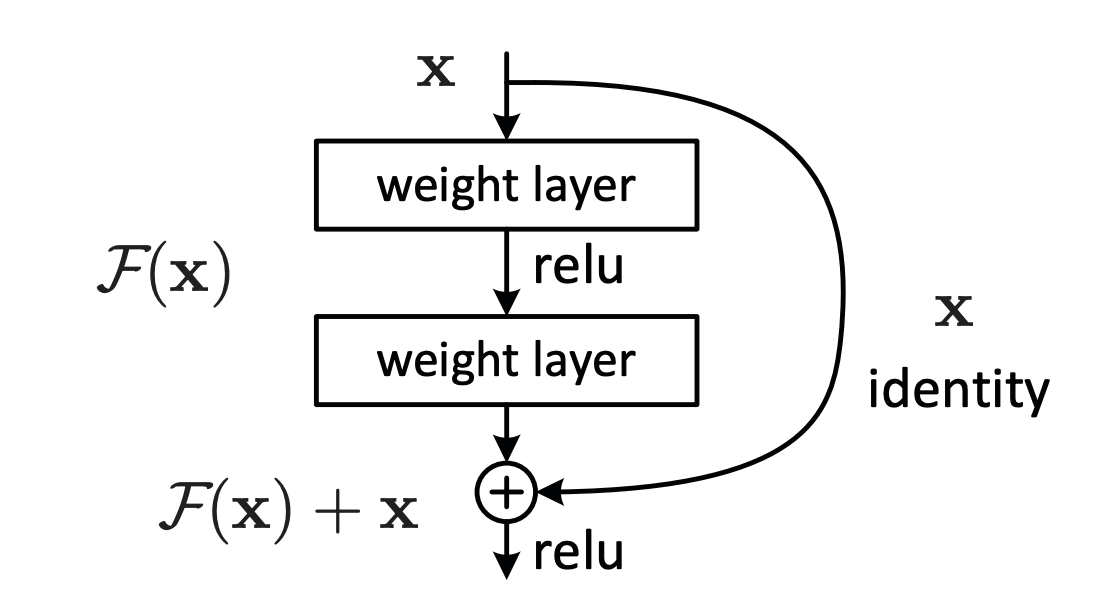
\includegraphics[width=0.5\textwidth]{images/appendix/blocks/resnet.png}
    \caption{Residual block architecture in the ResNet paper \cite{resnet}.}
    \label{fig:appendix_blocks_residual_block}
\end{figure}

Residual blocks (\texttt{ResBlock}) are skip-connection blocks that were introduced in the ResNet (Residual Network) paper \cite{resnet}. They are used to mitigate the \textbf{exploding/vanishing gradient problem} in very deep neural networks. A residual block allows the network to \textbf{skip layers} by adding identity shortcut connection (the input is added directly to the output of a few stacked layers). The main idea is that instead of learning the full mappings from input to output, the residual block only needs to learn a residual mapping (the difference between the input and output). Mathematically, residual mappings can be written as:

\begin{equation*}
    y = \mathcal{F} (x) + x
\end{equation*}

where $x$ is the input to the block, $\mathcal{F}$ is the residual function, and $y$ is the output of the block.

More importantly, if a layer doesn't need to transform the input, the skip connection allows the network to learn an identity mapping, making it easier to optimize the model. Easier flow of gradients also mitigate the problem of vanishing/exploding gradients, where the gradients become too small or too large as they are backpropagated through the network, as we add more and more stacked layers.

The architecture of a residual block is shown in figure \ref{fig:appendix_blocks_residual_block}. They are more commonly references as 'skip-connection' blocks.






\subsubsection{Normalization layers}
\label{appendix:blocks_norm}

These layers ensure that the data is normalized in a way that the model can learn better. If we think about optimizing our model on a distribution that looks like very long ellipse, it would be hard for the model to reach minima. But if we normalize the data such that the distribution will fit a circle, then the optimization process will be easier. 

For this topic we use mean $\mu$, variance (standard deviation) $\sigma$:

\[ \mu = \frac{1}{H} \sum_{i=1}^{H} x_i \]

\[ \sigma = \sqrt{\frac{1}{H} \sum_{i=1}^{H} (x_i - \mu)^2} \]

where $H$ is the number of elements in the input $x$.

\begin{figure*}
    \centering
    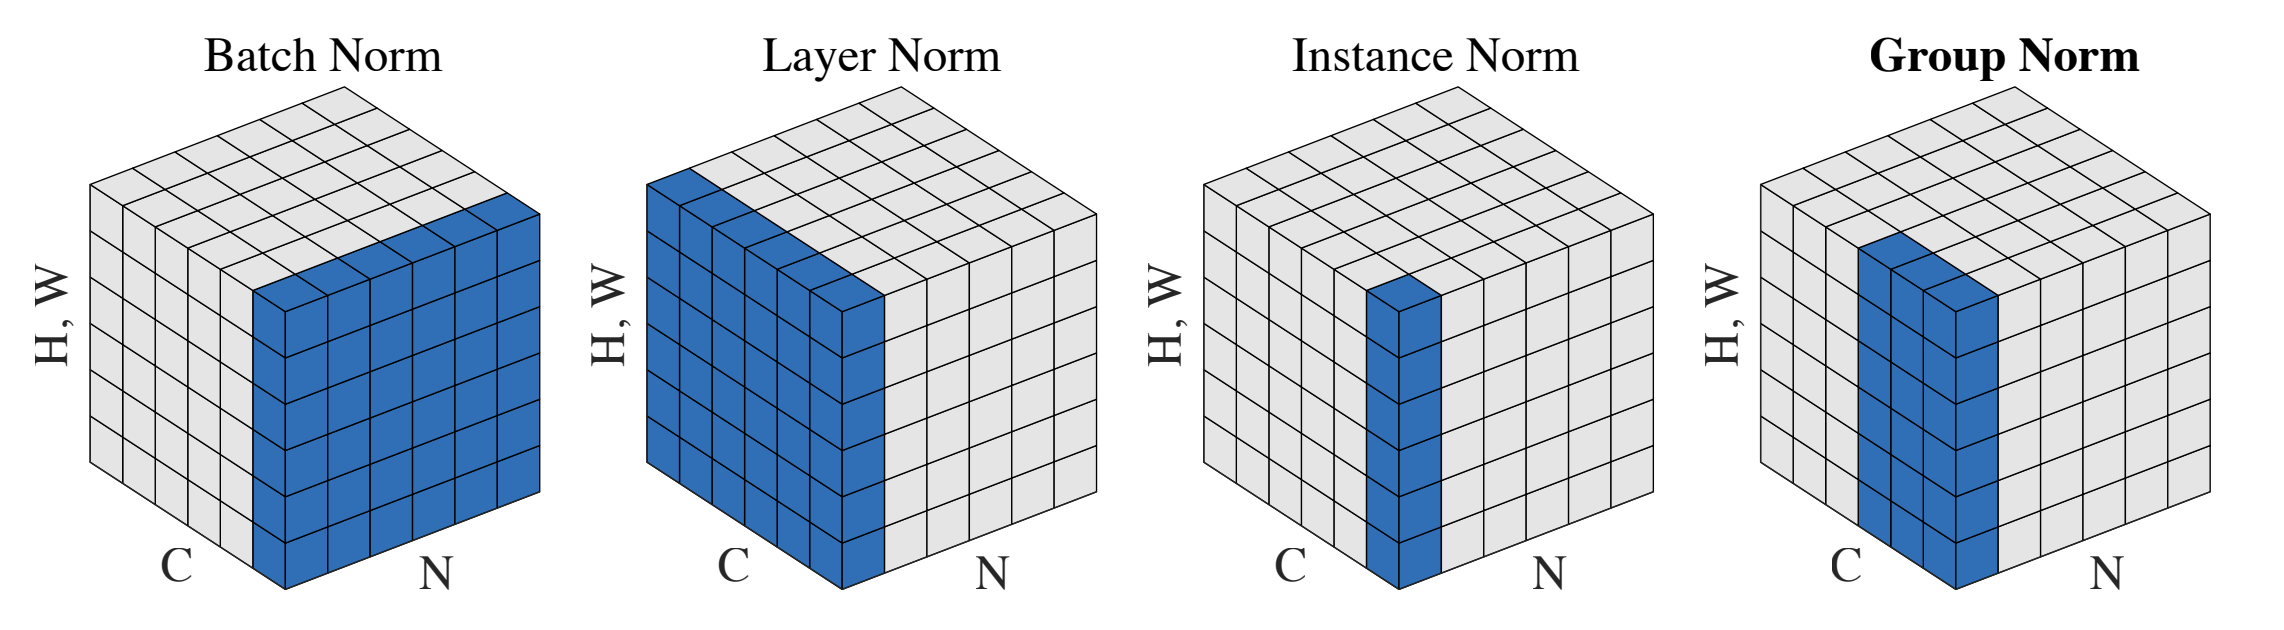
\includegraphics[width=0.75\textwidth]{images/appendix/blocks/norm.png}
    \caption{Visual comparison on mode of operations of \texttt{BatchNorm}, \texttt{LayerNorm}, \texttt{InstanceNorm}, \texttt{GroupNorm} where $N$ is the batch size, $C$ is the number of channels, $H,W$ is the height and width of the input. Image taken from "Group normalization" 2018 paper \cite{wu2018group}.}
    \label{fig:appendix_blocks_norm}
\end{figure*}

\subsection*{LayerNorm}

\texttt{LayerNorm} block is a normalization block that normalizes the input, which may be useful for stabilizing and accelerating the training process. It's introduced in a 2016 paper \cite{layernorm}. See figure \ref{fig:appendix_blocks_norm} for a visual demonstration.

\texttt{LayerNorm} normalizes the input across the feature channels, rather than across the batch (as in \texttt{BatchNorm} block). See figure \ref{fig:appendix_blocks_norm} for a visual comparison where \texttt{LayerNorm}, \texttt{BatchNorm} operates on each channel of the input.

It is defined as:

\begin{equation*}
    \text{LayerNorm}(x) = \frac{x - \mu}{\sqrt{\sigma^2 + \epsilon}} \cdot \gamma + \beta
\end{equation*}

where $\mu = \mathbb{E}(x)$ is the mean of the input, $\sigma = \text{Var} (x)$ is the variance of the input, $\epsilon$ is a small constant to avoid division by zero, and $\gamma, \beta$ are learnable parameters. The $\gamma$ and $\beta$ parameters scale and shift the normalized input.

Because \texttt{LayerNorm} doesn't rely on batch size, it can be applied even in batch size of 1.








\subsection*{BatchNorm}

Like \texttt{LayerNorm}, \texttt{BatchNorm} is a normalization block that speeds up training, decreases the importance of initial weights, and regularizes the model. It was introduced in a 2015 paper \cite{batchnorm}. A great YouTube video explaining why batch normalization speeds up the training process (by not overshooting in the learning rate) is available at \href{https://www.youtube.com/watch?v=DtEq44FTPM4}{this link}. See figure \ref{fig:appendix_blocks_norm} for a visual demonstration.

Let $\mu_B$ be the mean of the mini-batch, and $\sigma^2_B$ be the variance of the mini-batch, and $m$ be the number of samples in the mini-batch. The operation of \texttt{BatchNorm} is defined as:

\begin{equation*}
    \text{BatchNorm}(x) = \frac{x - \mu_B}{\sqrt{\sigma^2_B + \epsilon}} \cdot \gamma + \beta
\end{equation*}

where $\gamma, \beta$ are learnable parameters, and $\epsilon$ is a small constant to avoid division by zero. The $\gamma$ and $\beta$ parameters scale and shift the normalized input.








\subsection*{GroupNorm}

Similar to \texttt{LayerNorm} and \texttt{BatchNorm}, \texttt{GroupNorm} is a normalization block that normalizes the input but across the feature channels. It was introduced in a 2018 paper \cite{wu2018group}. \texttt{GroupNorm} strikes a balance between \texttt{LayerNorm} and \texttt{BatchNorm}, where it normalizes the input across the feature channel but not all of it, it normalizes groups of input features, hence the name. See figure \ref{fig:appendix_blocks_norm} for a visual demonstration.

Similar to \texttt{LayerNorm}, the operation of \texttt{GroupNorm} is defined as:

\begin{equation*}
    \text{GroupNorm}(x) = \frac{x - \mu}{\sqrt{\sigma^2 + \epsilon}} \cdot \gamma + \beta
\end{equation*}

where $\mu = \mathbb{E}(x)$ is the mean of the input, $\sigma = \text{Var} (x)$ is the variance of the input, $\epsilon$ is a small constant to avoid division by zero, and $\gamma, \beta$ are learnable parameters. The $\gamma$ and $\beta$ parameters scale and shift the normalized input.




\subsection*{Adaptive Layer Normalization (adaLN)}

% TODO: Complete
Adaptive Layer Normalization (adaLN) blocks are ...






\subsection{3D Convolutions}
\label{appendix:blocks_3dconv}

\begin{figure}
    \centering
    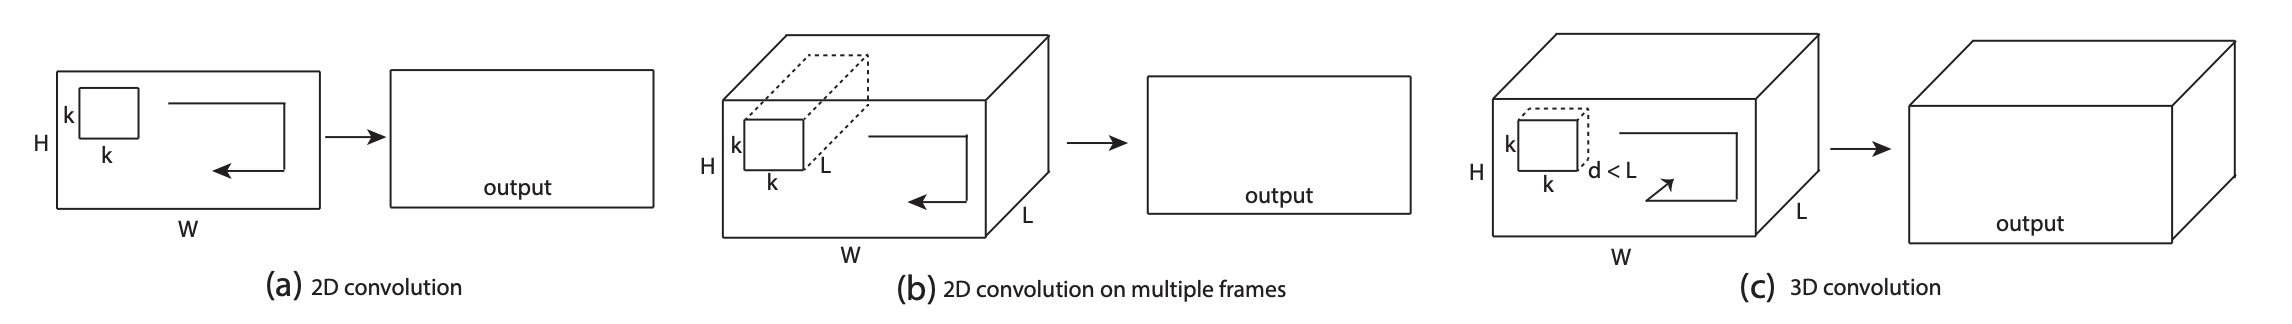
\includegraphics[width=1\textwidth]{images/appendix/blocks/3d_conv.png}
    \caption{2D and 3D convolution operations. (a) Applying 2D convolution on image results in an image. (b) Applying 2D convolution on video (multiple frames) also results in an image. (c) Applying 3D convolution on video results in another volume (channel), preserving temporal information. Figure from the 2014 paper \cite{tran2015learning}.}
    \label{fig:appendix_blocks_3dconv}
\end{figure}

The 2D and 3D convolution operation is demonstrated in figure \ref{fig:appendix_blocks_3dconv}.

3D convolution is an extension of the 2D convolutions but designed to fit into the 3D space (additional dimension, for video synthesis we can think of the third dimension as the \textbf{time dimension}).

Typically 2D convolutions have width, height dimension, and 3D convolutions have depth dimension which is suited to deal with temporal data, like videos. The 3D convolution kernels are also 3D. The extra dimension doesn't have to be time, in MRI imaging tasks, it can be the depth of the scan.

Lets consider an input of dimension $H \times W \times D$ and kernel of dimension $k_h \times k_w \times k_d$, then the kernel moves in all three dimensions and compute the sum of element-wise multiplication:

\begin{equation*}
    y_{i,j,k} = \sum_{l=0}^{k_d} \sum_{m=0}^{k_h} \sum_{n=0}^{k_w} x_{i+m,j+n,k+l} \cdot w_{m,n,l}
\end{equation*}

Just like 2D convolution, 3D convolution can have stride, padding and dilation. \textbf{Stride} is the number of steps the kernel moves in each dimension, \textbf{padding} is the number of zeros (padding) added to the input to maintain the output size, and \textbf{dilation} is the spacing between kernel elements.

In 2D convolution we have \texttt{in\_channels} and \texttt{out\_channel}, usually for images that are RGB encoded, the \texttt{in\_channels} is 3 (for red, green, blue channels) and the \texttt{out\_channels} represent the number of filters/kernels we want to apply. In 3D convolution, we have similar situation. 
